%% LyX 2.2.1 created this file.  For more info, see http://www.lyx.org/.
%% Do not edit unless you really know what you are doing.
\documentclass[10pt]{beamer}\usepackage[]{graphicx}\usepackage[]{color}
%% maxwidth is the original width if it is less than linewidth
%% otherwise use linewidth (to make sure the graphics do not exceed the margin)
\makeatletter
\def\maxwidth{ %
  \ifdim\Gin@nat@width>\linewidth
    \linewidth
  \else
    \Gin@nat@width
  \fi
}
\makeatother

\definecolor{fgcolor}{rgb}{0.345, 0.345, 0.345}
\newcommand{\hlnum}[1]{\textcolor[rgb]{0.686,0.059,0.569}{#1}}%
\newcommand{\hlstr}[1]{\textcolor[rgb]{0.192,0.494,0.8}{#1}}%
\newcommand{\hlcom}[1]{\textcolor[rgb]{0.678,0.584,0.686}{\textit{#1}}}%
\newcommand{\hlopt}[1]{\textcolor[rgb]{0,0,0}{#1}}%
\newcommand{\hlstd}[1]{\textcolor[rgb]{0.345,0.345,0.345}{#1}}%
\newcommand{\hlkwa}[1]{\textcolor[rgb]{0.161,0.373,0.58}{\textbf{#1}}}%
\newcommand{\hlkwb}[1]{\textcolor[rgb]{0.69,0.353,0.396}{#1}}%
\newcommand{\hlkwc}[1]{\textcolor[rgb]{0.333,0.667,0.333}{#1}}%
\newcommand{\hlkwd}[1]{\textcolor[rgb]{0.737,0.353,0.396}{\textbf{#1}}}%
\let\hlipl\hlkwb

\usepackage{framed}
\makeatletter
\newenvironment{kframe}{%
 \def\at@end@of@kframe{}%
 \ifinner\ifhmode%
  \def\at@end@of@kframe{\end{minipage}}%
  \begin{minipage}{\columnwidth}%
 \fi\fi%
 \def\FrameCommand##1{\hskip\@totalleftmargin \hskip-\fboxsep
 \colorbox{shadecolor}{##1}\hskip-\fboxsep
     % There is no \\@totalrightmargin, so:
     \hskip-\linewidth \hskip-\@totalleftmargin \hskip\columnwidth}%
 \MakeFramed {\advance\hsize-\width
   \@totalleftmargin\z@ \linewidth\hsize
   \@setminipage}}%
 {\par\unskip\endMakeFramed%
 \at@end@of@kframe}
\makeatother

\definecolor{shadecolor}{rgb}{.97, .97, .97}
\definecolor{messagecolor}{rgb}{0, 0, 0}
\definecolor{warningcolor}{rgb}{1, 0, 1}
\definecolor{errorcolor}{rgb}{1, 0, 0}
\newenvironment{knitrout}{}{} % an empty environment to be redefined in TeX

\usepackage{alltt}
\usepackage[T1]{fontenc}
\setcounter{secnumdepth}{3}
\setcounter{tocdepth}{3}
\usepackage{url}
\usepackage{graphicx}
\usepackage{adjustbox} % for \adjincludegraphics
\usepackage{booktabs}
\graphicspath{{/srv/shiny-server/prc/report/figure}}
\usepackage[font={footnotesize,it}]{caption}
%\ifx\hypersetup\undefined
    %\AtBeginDocument{%
        %\hypersetup{unicode=true,pdfusetitle,
            %bookmarks=true,bookmarksnumbered=false,bookmarksopen=false,
        %breaklinks=false,pdfborder={0 0 0},pdfborderstyle={},backref=false,colorlinks=false}
    %}
%\else
    %\hypersetup{unicode=true,pdfusetitle,
        %bookmarks=true,bookmarksnumbered=false,bookmarksopen=false,
    %breaklinks=false,pdfborder={0 0 0},pdfborderstyle={},backref=false,colorlinks=false}
%\fi
%\usepackage{breakurl}

\makeatletter

%%%%%%%%%%%%%%%%%%%%%%%%%%%%%%% LyX specific LaTeX commands.
%\providecommand{\LyX}{\texorpdfstring%
    %{L\kern-.1667em\lower.25em\hbox{Y}\kern-.125emX\@}
%{LyX}}

%%%%%%%%%%%%%%%%%%%%%%%%%%%%%%% Textclass specific LaTeX commands.
%% this default might be overridden by plain title style
%\newcommand\makebeamertitle{\frame{\maketitle}}%
%% (ERT) argument for the TOC
%\AtBeginDocument{%
    %\let\origtableofcontents=\tableofcontents
    %\def\tableofcontents{\@ifnextchar[{\origtableofcontents}{\gobbletableofcontents}}
    %\def\gobbletableofcontents#1{\origtableofcontents}
%}

%%%%%%%%%%%%%%%%%%%%%%%%%%%%%% User specified LaTeX commands.
\usetheme{PaloAlto}

\makeatother
\IfFileExists{upquote.sty}{\usepackage{upquote}}{}
\begin{document}


\title[knitr, Beamer, and FragileFrame]{Briefing of PRC Project}

\author{PRC Team\thanks{I thank everyone present at this moment.}}
\maketitle


\begin{frame}{Background}

    \begin{itemize}
        \item \textbf{Aim 1:} Develop procedures for rapid optimization and validation of "Personalized-Reference Chart" (PRC) algorithms for:
            \begin{itemize}
                \item Knee function
                \item Physical Function, and
                \item Patient-reported function
            \end{itemize}
        \item \textbf{Aim 2:} Develop a software application that generates PRCs and integrates with clinical practice
        \item \textbf{Aim 3:} Examine the implementation of PRCs in clinical practice via a feasibility study framework
    \end{itemize}

\end{frame}

\section{First Test}



%\begin{frame}[fragile]{First Test}
\begin{frame}{Method}




%latex.default(., booktabs = TRUE, file = "", title = "", table.env = FALSE,     size = "scriptsize", col.just = c("c", rep("p{1.8in}", 2)),     rowname = NULL)%
{\scriptsize
\begin{center}
\begin{tabular}{cp{1.8in}p{1.8in}}
\toprule
\multicolumn{1}{c}{Steps}&\multicolumn{1}{c}{Description}&\multicolumn{1}{c}{Modeling}\tabularnewline
\midrule
$1$&Splitting of training and testing data&Train-Test Split\tabularnewline
$2$&Fitting of model to predict clinically relevant outcome (e.g. 90 day post-operative TUG)&Linear Mixed Model w/ b-spline\tabularnewline
$3$&Fitting of model based on variables that contribute significantly to the previously predicted outcome&General Linear Model\tabularnewline
$4$&Matching of patients based on the fitted/predicted value generated from the genera linear model&Nearest N Matching\tabularnewline
$5$&Leave one out cross validation to obtain measures of bias, coverage, and precision&LOOCV\tabularnewline
$6$&Based on optimal number of matches, predict on test set&Generalized Additive Model for Location, Scale, and Shape\tabularnewline
\bottomrule
\end{tabular}\end{center}}


%BTW, the first element of \texttt{x} is x[1]. (Did you notice the use of\texttt{ \textbackslash{}Sexpr\{\}}?)
\end{frame}

\section{Result}
\begin{frame}[fragile]{Table 1}




\begin{table}

\caption{\label{tab:tab1}Table 1. Baseline Characteristics of Training and Testing Set}
\centering
\resizebox{\linewidth}{!}{
\begin{tabular}[t]{lccr}
\toprule
  & Test & Train & p\\ & (N = 202, \# TUG Obs = 604) & (N = 397, \# TUG Obs = 1339) &  \\
\midrule

Age (years) (mean (sd)) & 65.90 (8.84) & 64.04 (8.43) & 0.012\\
Gender = Male (\%) & 84 (41.6) & 185 (46.6) & 0.280\\
BMI (kg/m\textasciicircum{}2) (mean (sd)) & 31.98 (6.20) & 31.33 (5.82) & 0.208\\
Baseline TUG (sec) (mean (sd)) & 11.00 (5.04) & 9.98 (4.95) & 0.018\\
\bottomrule
\end{tabular}}
\end{table}



\end{frame}


\begin{frame}{Figure 2}

\begin{figure}[!htbp]
\centering
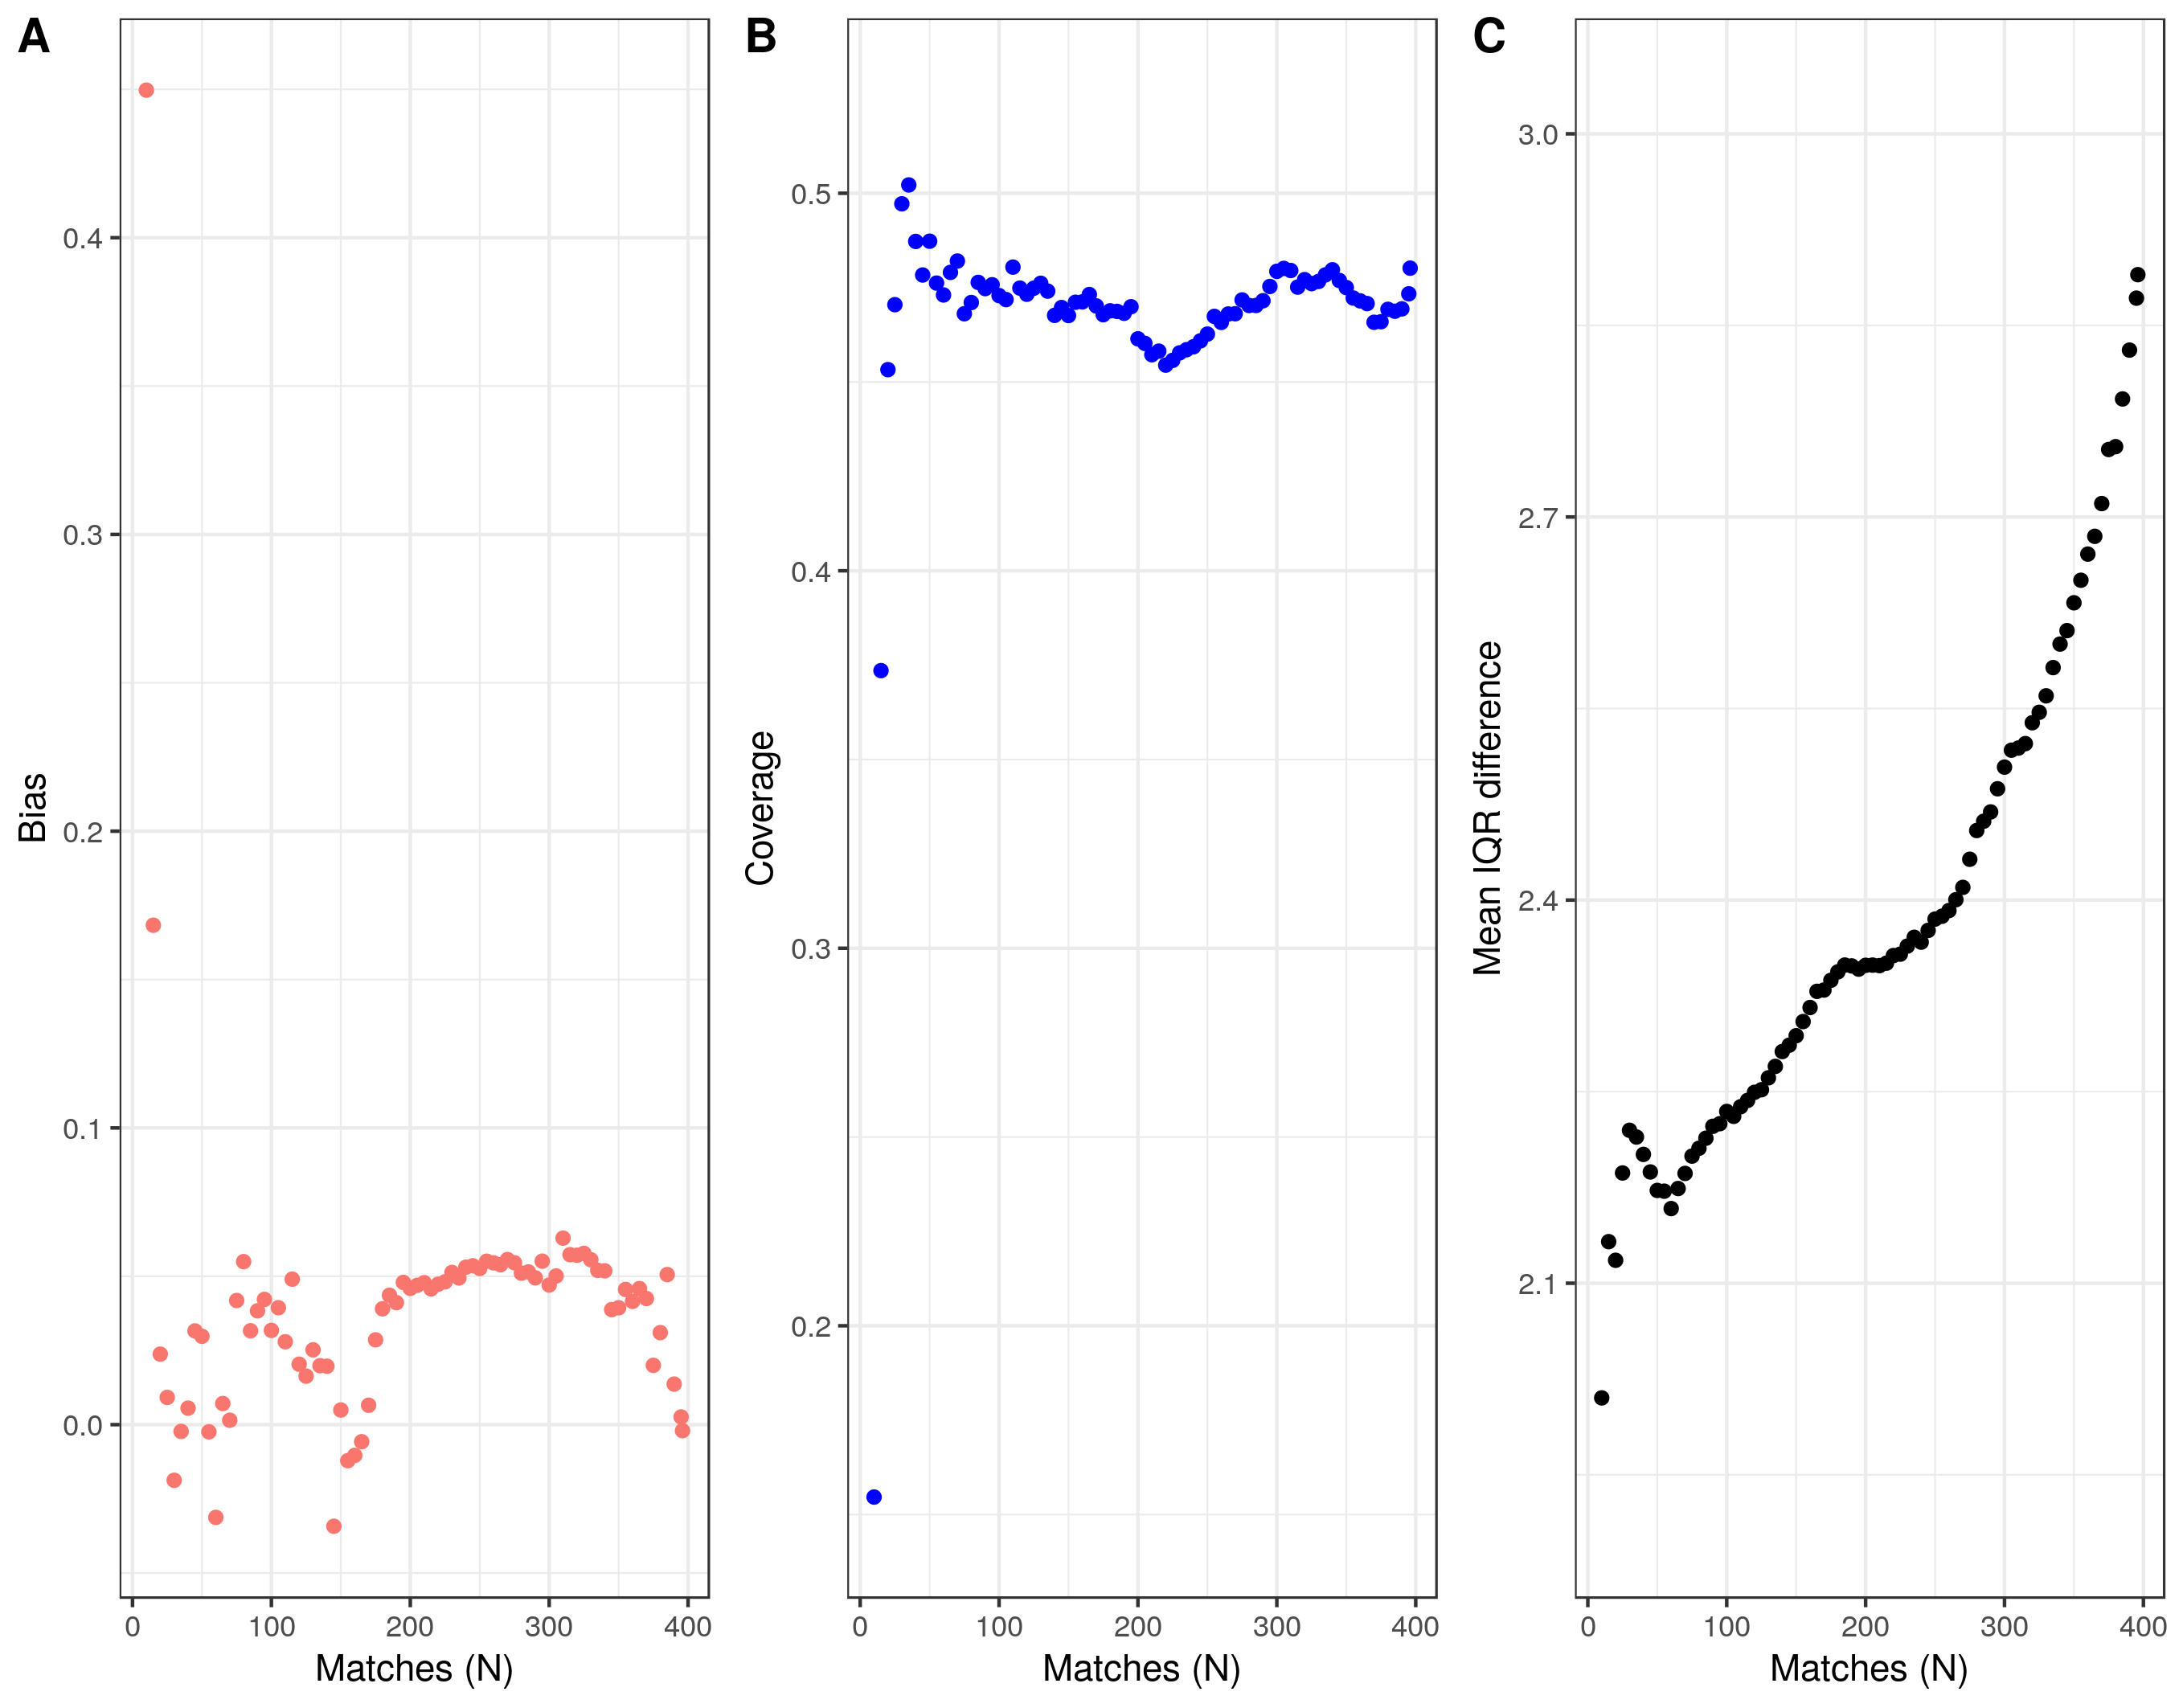
\includegraphics[width=0.85\linewidth]{../figure/fig_BCPEo_loocv}
\caption{Bias, Precision, and Coverage plot using Box-Cox-Power-Exponential distribution for location, shape, and scale for gamlss}
\label{fig:fig_BCPEo_loocv}
\end{figure}

\end{frame}


\begin{frame}{Figure 3}

\begin{figure}[!htbp]
\centering
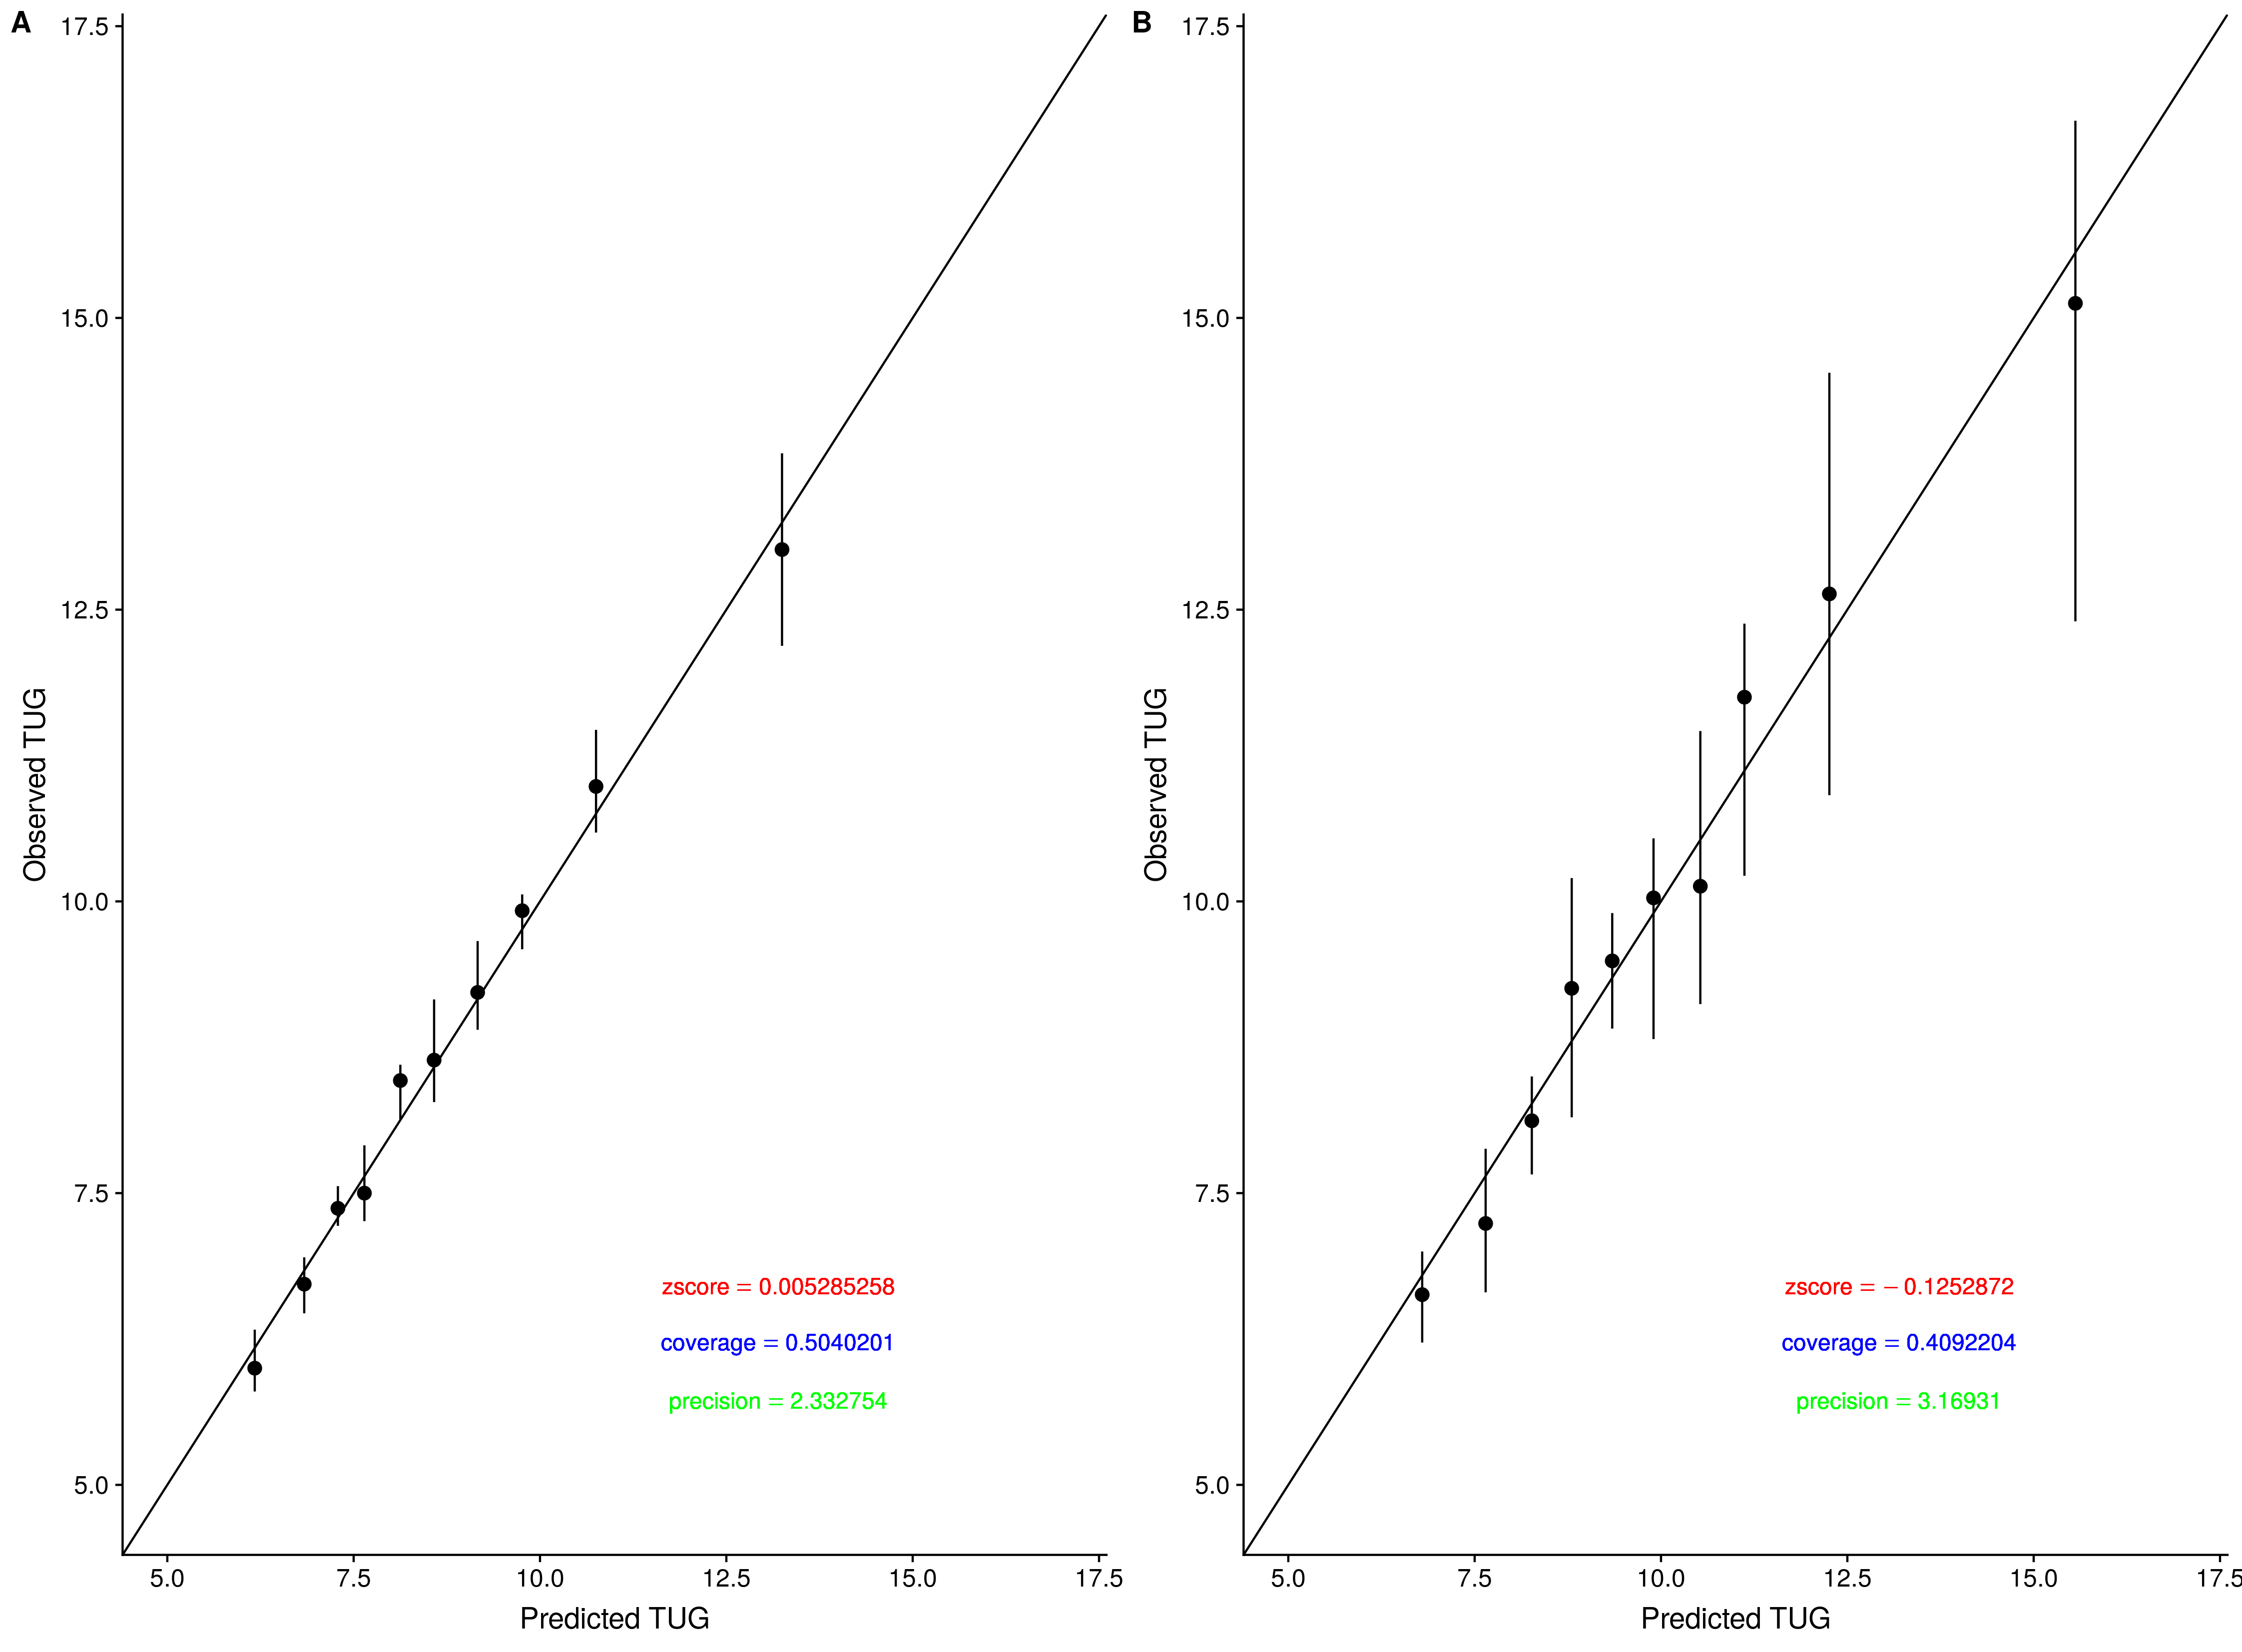
\includegraphics[width=0.85\linewidth]{../figure/fig_BCCGo_cal}
\caption{Calibration plot of N = 35 matches using Box-Cox-Cole-Green distribution for location, shape, and scale for gamlss}
\label{fig:fig_BCCGo_cal}
\end{figure}

\end{frame}


\begin{frame}{Figure 4: Zoom In}

\begin{figure}[!htbp]
\centering
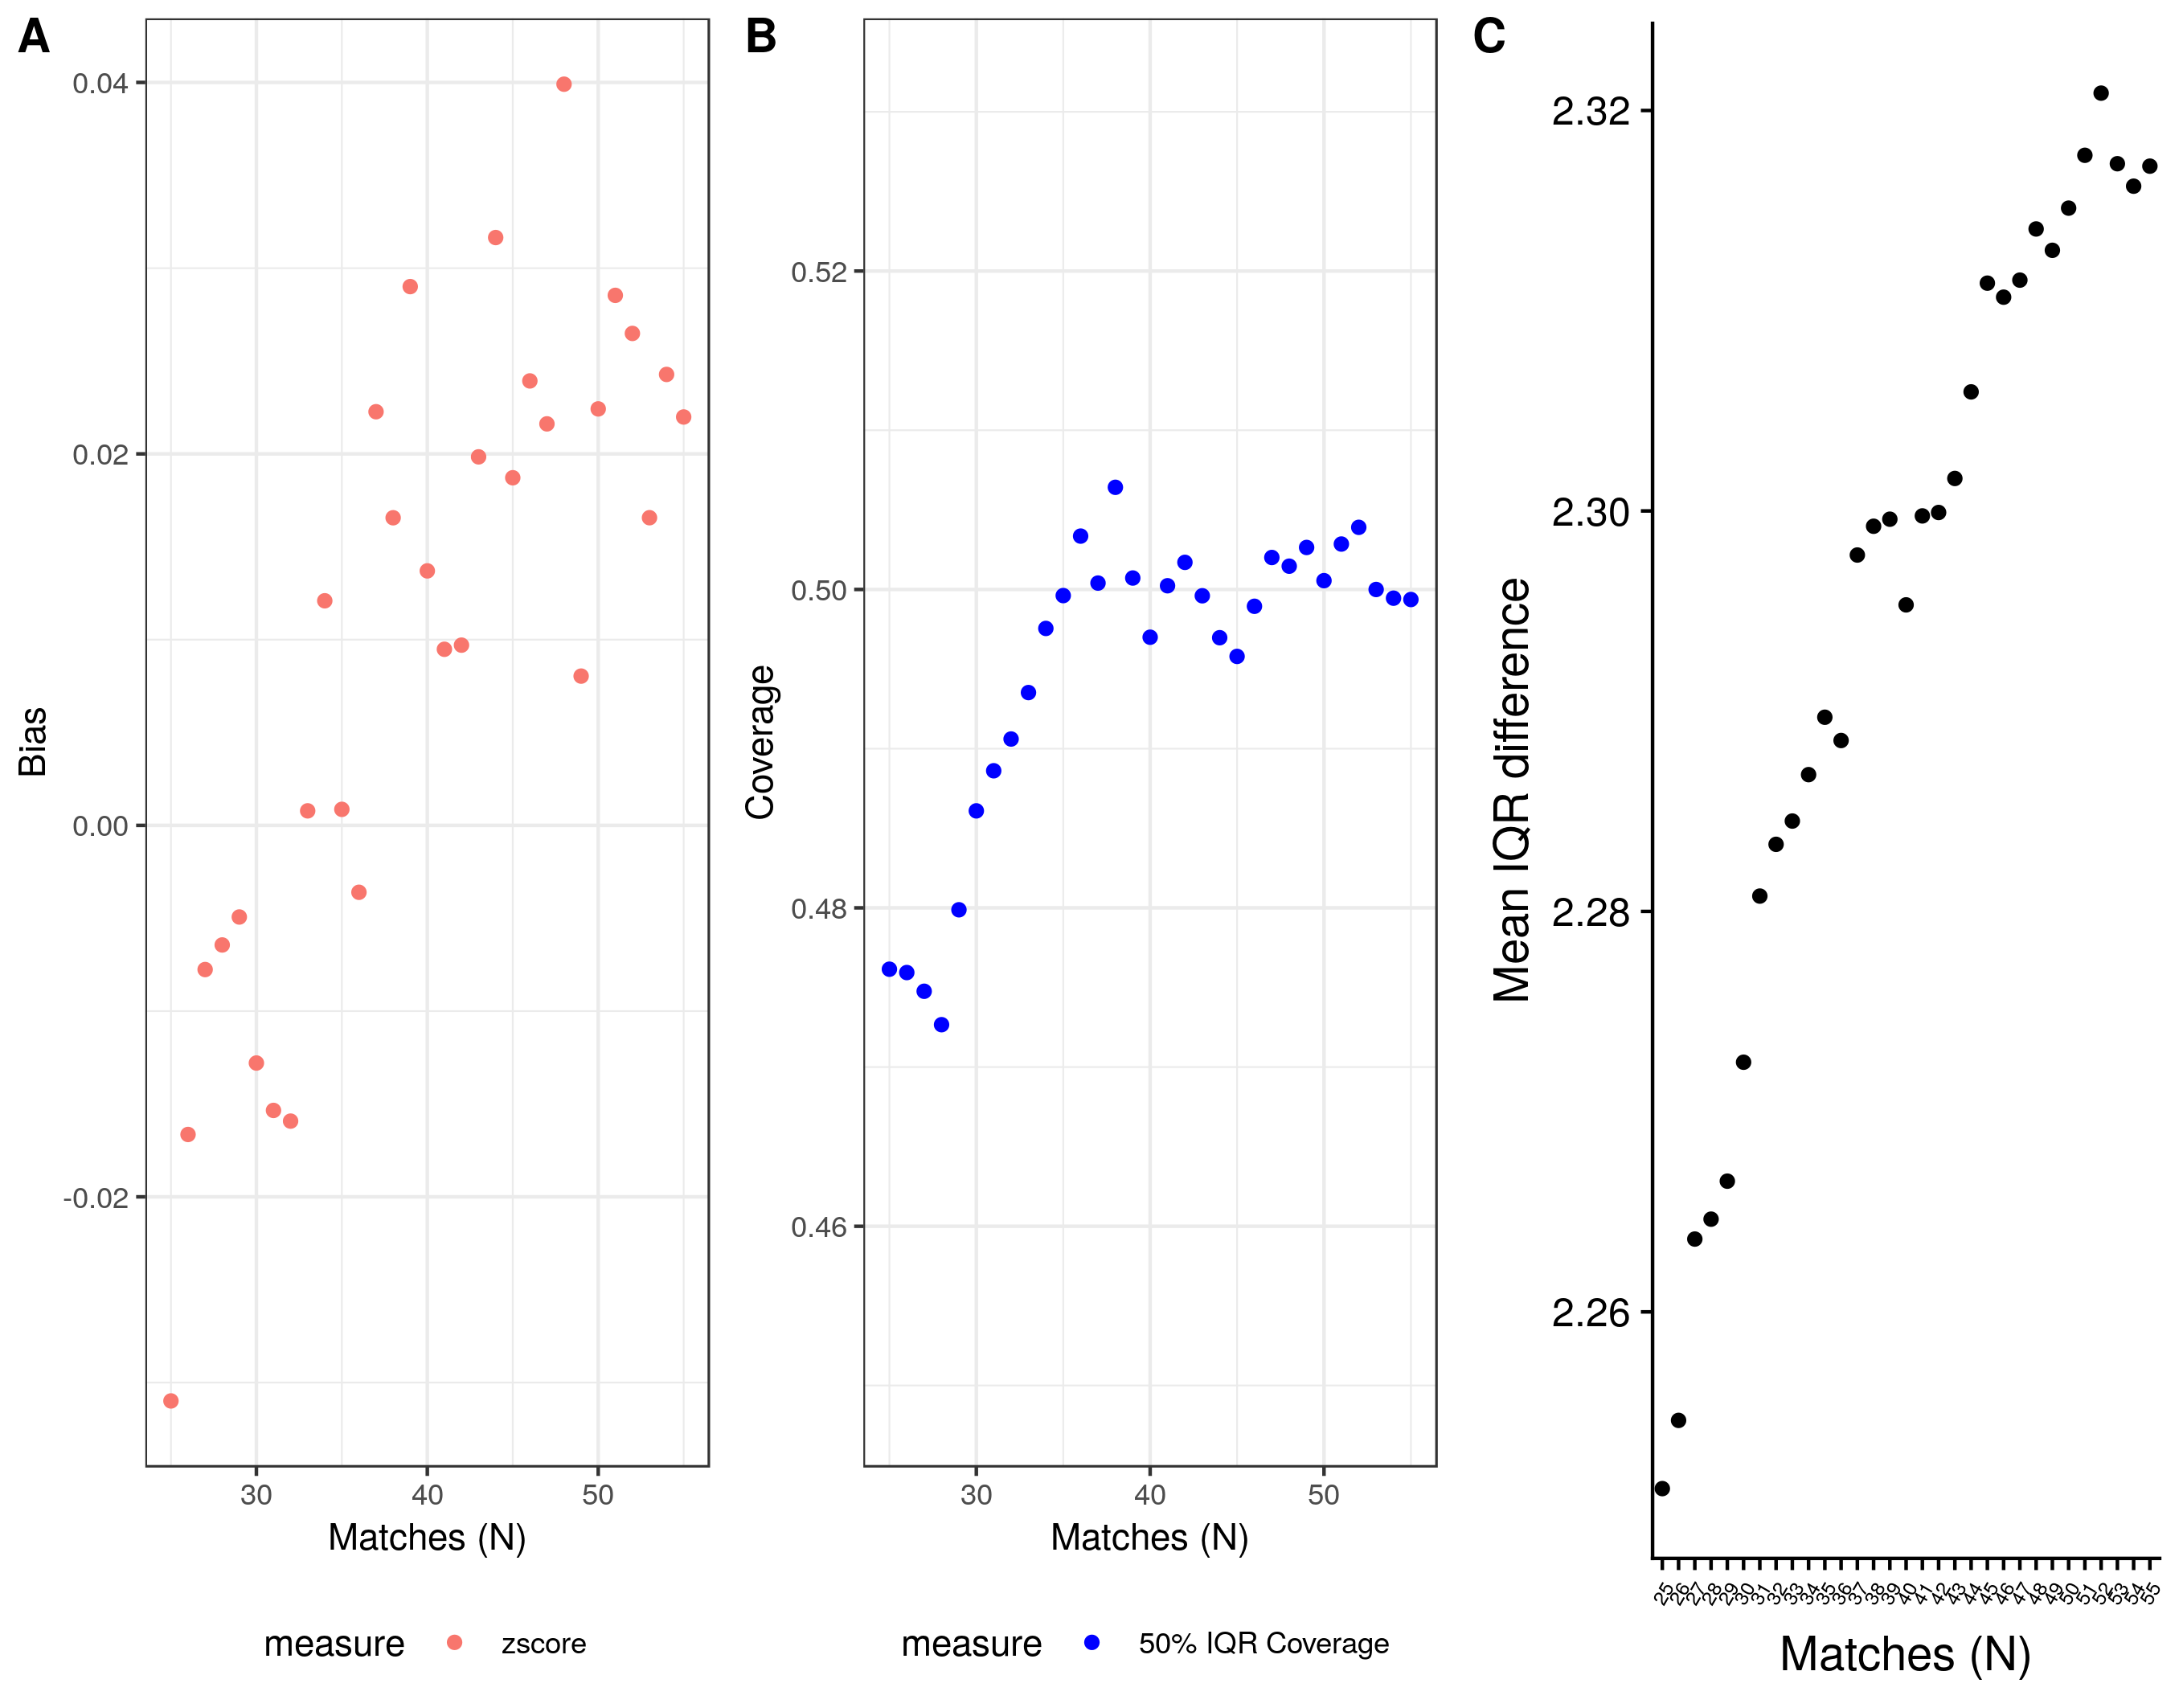
\includegraphics[width=0.85\linewidth]{../figure/fig_BCCGop_loocv}
\caption{Bias, Precision, and Coverage plot using Box-Cox-Cole-Green distribution for location, shape, and scale for gamlss; Zoomed In}
\label{fig:fig_BCCGo_cal}
\end{figure}

\end{frame}


\end{document}
